\chapter{Fonctionnement interne}
\section*{Introduction}
La composé principal des composants électronique est le silicium car celui-ci est
un semi-conducteur, un corps aux propriétés entre celle d'un bon conducteur et 
d'un isolant. Quel est l'itnérêt de travailler avec un mauvais conducteur/isolant? 
Car on parvient à modifier la conductivité de manière électrique : on peut 
imposer la valeur d'un courant et créer nos fameux circuits.

\section{Physique des semi-conducteurs}
	\subsection{Solides conducteurs : courant électrique}
			\begin{wrapfigure}[8]{r}{3cm}
		\vspace{-0.5cm}
		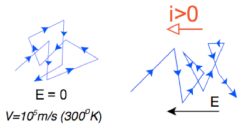
\includegraphics[scale=0.35]{ch6/image1}
		\captionof{figure}{ }
		\end{wrapfigure}
	Considérons une température non nulle de 300K. Si l'on applique pas de courant, 
	l'agitation thermique cause un mouvement aléatoire comme on aurait pour un 
	gaz\footnote{Les mouvements individuels s'annulent.} : $I_{net} = 0$. \\
	Par contre, l'application d'une ddp crée un champ électrique attirant les 
	électrons dans une direction : le mouvement est toujours désordonné mais il 
	existe une direction préférentielle et donc $I_{net}>0$.

	\subsection{Cristal de Si (pur)}
			\begin{wrapfigure}[8]{l}{8cm}
		\vspace{-0.5cm}
		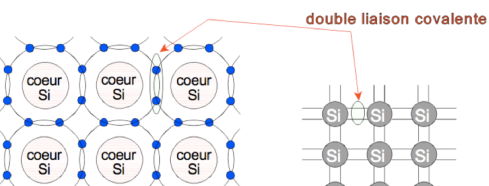
\includegraphics[scale=0.4]{ch6/image2}
		\captionof{figure}{ }
		\end{wrapfigure}	
	Intéressons nous à ce fameux cristal, qui possède une structure atomique 
	différente : moins de couches électroniques 4 $e^-$ de valence au lieu d'un 
	et une charge de cœur (cœur : noyau + couches internes) plus grande.  Il 
	est alors possible de les arranger comme les métaux en complétant la couche 
	périphérique pour avoir huit électrons $\rightarrow$ 8 liaisons covalentes.\\
	
	Les métaux n'utilisent \textbf{pas} la liaison covalente, consistant en la mise en 
	commun d'un électron de deux atomes. Comme $Si$ possède 4 $e^-$ périphérique 
	il peut se lier à 4 atomes voisins pour avoir une couche périphérique de 8 
	$e^-$.\\
	Tous les électrons de valences sont tous "utilisés"/"bloqués" par les liaisons 
	covalentes mais ils sont aussi plus "liés" que dans un atome de métal car 
	le $Si$ possède moins de couche : l'attraction du 	noyau est plus forte. De 
	plus le cœur est plus chargé : encore plus d'attraction.\\
	
	Tout ceci montre que l'énergie de liaison est bien plus forte que dans un 
	métaux, il en résulte une faible conductivité.\\
	
			\begin{wrapfigure}[12]{l}{8.5cm}
		\vspace{-0.5cm}
		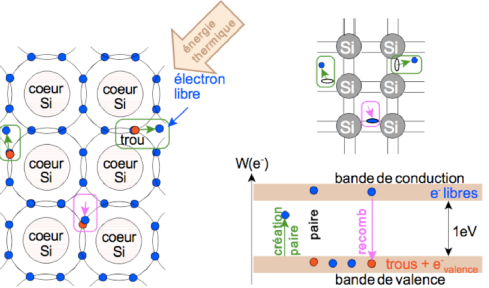
\includegraphics[scale=0.47]{ch6/image3}
		\captionof{figure}{ }
		\end{wrapfigure}	
	La seconde grande différence est que si un électron se fait arracher (pour 
	devenir une charge libre dans la bande de conduction), il 
	laisse un "trou" à sa place, soit un défaut d'électron ; par rapport à l'
	atome neutre, c'est une charge positive. La libération d'un électron 
	crée automatiquement une paire électron/trou : tous deux peuvent se 
	déplacer pour former du courant. On parle de recombinaison électron-trou 
	quand un électron vient combler un trou. Si un trou est comblé par un 
	électron de valence d'une liaison adjacente, il laisse à son tour un nouveau 
	trou : le déplacement de l'$e^-$ provoque le déplacement d'un trou, une 
	charge positive susceptible 	de se déplacer\footnote{Un électron possède 
	une mobilité triple qu'un trou, et donc un courant bien plus important.}.



	\subsection{Dopage}
	La différence entre un semi-conducteur est un bon conducteur est que sa 
	conductivité est bien plus faible et qu'il possède deux types de charges. 
	Le \textit{dopage}, c'est ajouter volontairement des impuretés (atomes 
	étrangers) pour augmenter grandement la conductivité du matériau.
		
		\subsubsection{Atome donneur/accepteur}
		Le but est d'introduire un atome pentavalent à la place d'un atome de 
		silicium : un électron de valence ne participe pas aux liaisons 
		covalentes et est quasiment libre au point de participer à la conduction. 
		Il s'agit donc d'un atome donneur. L'inverse est également faisable en 
		introduisant un atome trivalent : un quasi-trou (car son énergie est 
		très proche de celle d'un électron de valence) sera créé et il peut 
		participer à la conduction. On parle alors d'atome accepteur.\\
		Il existe alors deux types de dopages :
		\begin{enumerate}
		\item Semi-conducteur \textbf{intrinsèque} : propriétés dépendent 
		uniquement de ses caractéristiques propres (Si pur, Si dopé à haute 
		température, \dots)
		\item Semi-conducteur \textbf{extrinsèque} : propriété dépendent 
		essentiellement du dopant (type P ou N).
		\end{enumerate}


		\subsubsection{Dopage par atome donneurs}
		L'introduction des donneurs donne un véritable "réservoir d'électrons" 
		facilement libéré par agitation thermique : un très petit nombre de 
		donneurs joue énormément sur la conductivité. On observe également une 
		diminution du nombre de trou. Le produit des densités $p*n$ est constant. Avec un 
		tel dopage, il y a environ $2*10^ 8$ fois plus d'$e^-$ que de trous. Les 
		$e^-$ sont majoritaires et les trous minoritaires.
		
		\subsubsection{Effet de la température}
		Le produit des densité de charges mobiles $n*p$ ne dépend \textbf{que} 
		de la température et grandit fortement avec elle 
		\begin{equation}
		pn \propto T^3e^{-\dfrac{W_G}{kT}}
		\end{equation}
		On remarque alors qu'au delà d'une certaine température (500K), $n>N_a,N_d$ 
		la densité de dopant : le Si redevient intrinsèque et on ne parle plus de 
		type p et n car toutes les propriétés acquises par le dopage sont perdues 
		(en effet, il y a suffisamment d'énergie thermique que pour faire passer 
		les électrons de valence dans la bande de conduction). Cependant, attention 
		à la surchauffe!
		
		\subsubsection{Synthèse (atomes donneurs)}
		Une faible quantité de dopage modifie à mort la composition des porteurs 
		mobiles : la densité des électrons devient celle des donneurs, ils deviennent 
		majoritaire et les trous minoritaires. On parle de semi-conducteurs de 
		\textbf{type n} car les charges négatives sont minoritaires.

		\subsubsection{Synthèse (atomes accepteurs)}
		Les conclusions sont inversées : trous majoritaires, électron minoritaire. On 
		parle de semi-conducteurs de \textbf{type p}.
		
		
\section{Jonction PN et diode}
	\subsection{Jonction PN}
	La jonction PN est la frontière entre deux blocs de semi-conducteurs accolés : 
	un de type P et un de type N (réalisé par un dopage sélectif du Si). C'est la 
	frontière entre les deux zones, aux propriétés particulières, qui est à la base
	même de l'électronique. Par exemple, la diode est une jonction PN aux 
	extrémités métallisées.
	\begin{center}
	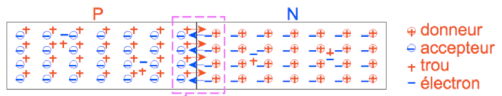
\includegraphics[scale=0.55]{ch6/image4}
	\captionof{figure}{ }
	\end{center}
	Si on connecte les jonctions P et N, à la frontière (jonction) les porteurs majoritaires 
	vont se recombiner et l’électro-neutralité n'est localement plus assurée car 
	il n'y a plus de charges mobiles pour compenser les charges fixes : la région P 
	se charge négativement et la région N positivement. Un champ électrique 
	va donc se créer (par la présence des charges fixes!), repoussant les porteurs 
	majoritaires et attirant les minoritaires.\\
	
	Cette zone, appauvrie en charges mobiles, est la \textbf{zone de charge d'espace}. 
	Elle ne contient plus que des charges fixes créant un champ repoussant les 
	porteurs majoritaires. On peut associer ce champ à une barrière de potentiel 
	empêchant les porteurs majoritaires à traverser la frontière entre les deux blocs.
		\begin{center}
	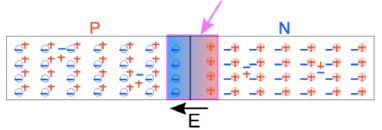
\includegraphics[scale=0.55]{ch6/image5}
	\captionof{figure}{ }
	\end{center}
	Nous avons créer un composant bloquant le passage du courant : diode à l'état 
	bloquant. Trouvons un moyen de la débloquer: c'est la polarisation.	
	
	\subsection{Jonction PN polarisée}
		 \subsubsection{Polarisation inverse (en sens bloquant)}
		 			\begin{wrapfigure}[4]{r}{3.5cm}
		\vspace{-0.8cm}
		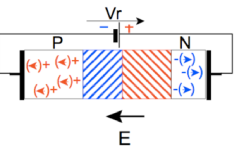
\includegraphics[scale=0.47]{ch6/image6}
		\captionof{figure}{ }
		\end{wrapfigure}	
		 On applique une tension \textbf{positive} du côté \textbf{N}. Le potentiel 
		 du côté N est plus positif que celui du côté P. Ceci éloigne les porteurs 
		 majoritaire de la jonction qui devient plus grande. Le pouvoir bloquant 
		 de la diode est renforcé par une polarisation négative.
		 
		 \subsubsection{Polarisation directe}
		\begin{wrapfigure}[6]{l}{4.5cm}
		\vspace{-0.5cm}
		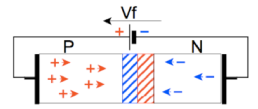
\includegraphics[scale=0.47]{ch6/image7}
		\captionof{figure}{ }
		\end{wrapfigure}
		 On applique un tension \textbf{positive} du coté \textbf{P}. Il y a donc 
		 une tendance à repousser les porteurs majoritaires vers la jonction et 
		 réduire la zone de charge d'espace. A un certain moment, la barrière devient 
		 plus faible à tel point que les porteurs majoritaires ont assez d'énergie 
		 que pour passer outre celle-ci : la diode devient passante. Les électrons 
		 et les trous se recombinent à la jonction, permettant au courant de circuler.
	
	
	
	\subsection{Caractéristique réelle d'une diode}
			\begin{wrapfigure}[8]{l}{8.5cm}
		\vspace{-0.5cm}
		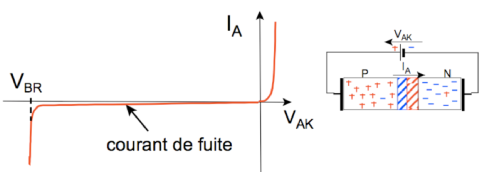
\includegraphics[scale=0.47]{ch6/image8}
		\captionof{figure}{ }
		\end{wrapfigure}
	Le coude de la caractéristique réelle d'une diode correspond au moment ou le potentiel 
	peut être contré par le champ extérieur : les porteurs peuvent passer et le courant 
	augmente. Considérons maintenant la polarisation en inverse. Les porteurs ayant 
	assez d'énergie pour franchir la barrière sont rare : s'ils passent ils sont 
	peu nombreux. Cela va générer des paires électrons/trous dans la jonction et 
	provoquer un courant de surface qui n'est rien d'autre que le courant de fuite.\\
	
	La bonne nouvelle est que l'on peut maintenant expliquer l'avalanche. En polarisation 
	inverse, les charges qui passent sont responsables d'un courant de fuite. Ces charges 
	ont un parcours chaotique et plus la tension est élevée plus ces charges vont vites 
	et créent des collisions rapides. L'avalanche résulte de deux collisions trop violentes :
	\begin{enumerate}
	\item Les collisions échauffent les atomes du cristal (destruction de la diode)
	\item Si tension inverse très importante, un électron accéléré peut arracher un 
	électron de valence et créer une paire électron-trou qui va lui aussi arracher\dots
	Il en résulte une augmentation du courant inverse de la dioe, diode incapable de 
	supporter ça.
	\end{enumerate}

















	
	

